\chapter{IPFS}
\label{ipfs}

IPFS\footnote{\url{https://ipfs.io/}} stands for Interplanetary File System and is a peer-to-peer distributed file system designed to make the Web faster, safer, and more open. In contrast with a standard file system, objects in IPFS are content-addressed by the cryptographic hash of their contents. In the case of the standard Web, when the user wants some file, he needs to know on which server is a file located and the full path to the file (see Figure \ref{webAddressing}). The principle of the IPFS is that a user needs only to know the hash of the requested file. He does not care about the location of the file (see Figure \ref{ipfsAddressing}). Let us take an MIT licence text, and add it to IPFS. If somebody tries to add this licence as a file to IPFS, it will return \texttt{QmWpvK4bYR7k9b1feM48fsk\-t2XsZfMaPfNnFxdbhJHw7QJ} every time. That is from now on the \textit{content address} of that file. Later, when a user tries to get this file by its hash, he can get it from a random person that added it into IPFS in the past.

IPFS can easily represent a file system consisting of files and directories. A~small file (less than 256 kB) is represented by an IPFS object with data being the file contents (plus a small header and footer). Note that the file name is not part of the IPFS object, so two files with different names and the same content will have the same IPFS object representation and hence the same hash. A~large file (more than 256 kB) is represented by a list of links to file chunks that are less than 256 kB, and only minimal information specifying that this object represents a large file. Currently, there are no known size limitations uploaded file or directory. There are already some big datasets hosted on IPFS such as Geocities archive\footnote{\url{https://ipfs.io/ipfs/QmVCjhoEFC9vwvaa8bKyJgwAByP4MXSogcyDGoz4Lkc3ox}} (704 TB) or Project Apollo Archives\footnote{\url{https://ipfs.io/ipfs/QmSnuWmxptJZdLJpKRarxBMS2Ju2oANVrgbr2xWbie9b2D}} (61 GB).


\begin{figure}[h]
    \centering
    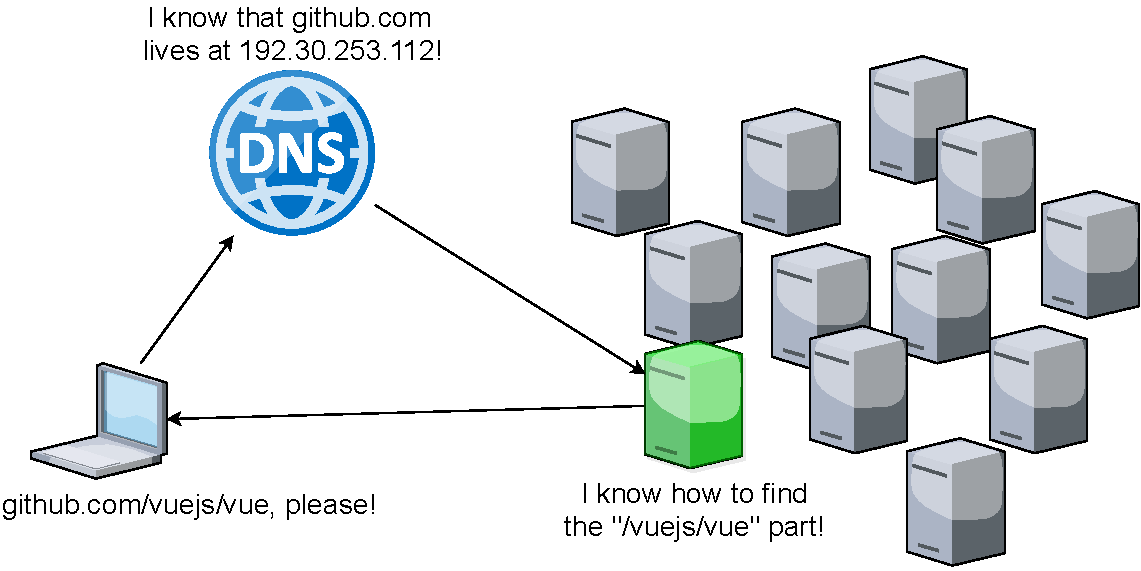
\includegraphics[width=11cm]{classicWebAddresing.pdf}
    \caption{Classic web addressing}
    \label{webAddressing}
\end{figure}

\begin{figure}[h]
    \centering
    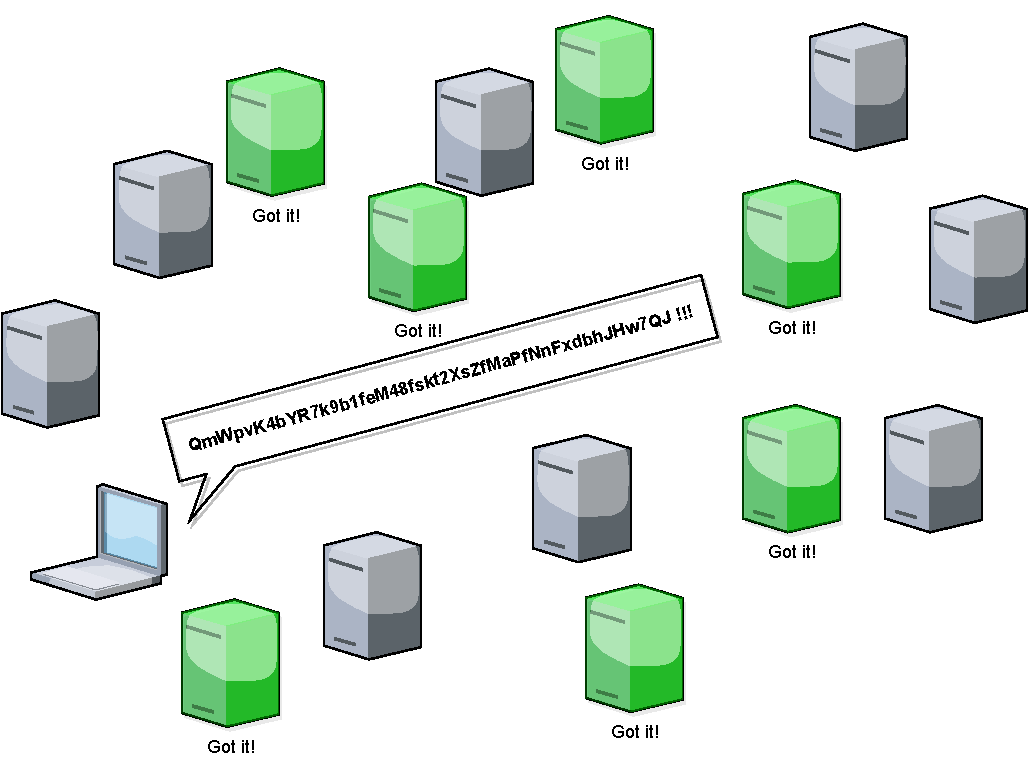
\includegraphics[width=11cm]{ipfsAddressing.pdf}
    \caption{Content-based addressing}
    \label{ipfsAddressing}
\end{figure}

\section{IPFS Stack}
We can split IPFS into layers (see Figure \ref{IPFSstack}). \textit{Libp2p}\footnote{\url{https://libp2p.io/}} is at the bottom, which is a peer-to-peer networking module, that handles peer and content discovery, transport, security, identity, peer routing, and messaging. \textit{IPLD} is the data model of the content-addressable web. It is providing linking between objects and multihash computing. On the top is \textit{IPFS}, which allows publishing and share files (or any data). \cite{IPFSwhitepaper}


\begin{figure}[h]
    \centering
    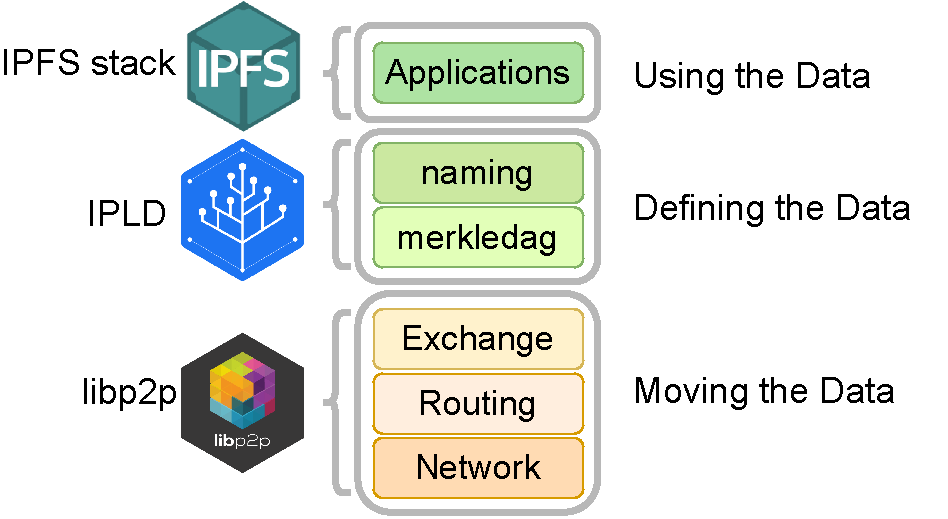
\includegraphics[width=11cm]{IPFSstack.pdf}
    \caption{IPFS stack}
    \label{IPFSstack}
\end{figure}


\section{Libp2p}
Libp2p is a modular system of protocols, specifications and libraries that enable the development of peer-to-peer network applications. It provides NAT Traversal, Peer Discovery, Routing, Stream Multiplexing, Protocol Multiplexing, Encryption, Authentication and more. It grew out of IPFS to solve networking problems in p2p networks, but now it does not require or depend on IPFS. Today many projects use libp2p as their network transporting layer, which is responsible for the actual transmission and receipt of data from one peer to another. For both content discovery and peer routing, libp2p uses Kademlia-based distributed hash table. With Kademlia, libp2p iteratively routes requests closer to the desired peer or content using Kademlia routing algorithm \cite{kademlia}. In the future, Kademlia might be changed easily to some other solution that implements a simple interface for publishing and requesting data and finding a peer. \cite{WebEngineering}


% \begin{figure}[h]
%     \centering
%     \begin{lstlisting}
%         // gets a particular peer's network address
%         FindPeer(node NodeId)

%         // stores a small metadata value in DHT
%         SetValue(key []bytes, value []bytes)

%         // retrieves small metadata value from DHT
%         GetValue(key []bytes)

%         // announces this node can serve a large value
%         ProvideValue(key Multihash)

%         // gets a number of peers serving a large value
%         FindValuePeers(key Multihash, min int)

%     \end{lstlisting}
%     \caption{libp2p interface}
%     \label{libp2pInterface}
% \end{figure}

\section{IPLD}
IPLD is providing linking and addressing objects with CID (Content ID). CID is hash-based self-describing content identifier (usually encoded to base58\footnote{\url{https://en.wikipedia.org/wiki/Base58}} format) which includes codec and multihash. Multihash is then further composed of hash type and hash value. Let us look closer on the MIT licence file, that we add to IPFS at the beginning of this chapter (see Figure \ref{ipfs}). Its CID is \texttt{QmWpvK4bYR7k9b1feM48fsk\-t2XsZfMaPfNnFxdbhJHw7QJ}. It can be converted to human-readable format as can be seen in Figure \ref{tab:CIDexample}, thanks to multicodec table\footnote{\url{https://github.com/multiformats/multicodec/blob/master/table.csv}}. We can see that this CID is encoded in base58 format and the file was stored using protobuf\footnote{\url{https://en.wikipedia.org/wiki/Protocol\_Buffers}} codec (this information is necessary to decode file correctly).



\begin{table}[]
    \centering
    \begin{tabular}{|ll|l|}
    \hline
    \textbf{Property}                  &             & \textbf{Value}                                                            \\ \hline
    Multibase                                        &             & base58btc                                                        \\ \hline
    Version                                          &             & cidv0                                                            \\ \hline
    Multicodec                                       &             & dag-pb                                                           \\ \hline
    \multicolumn{1}{|l|}{\multirow{3}{*}{Multihash}} & Hash Type   & sha2-256                                                         \\ \cline{2-3} 
    \multicolumn{1}{|l|}{}                           & Hash Length & 256                                                              \\ \cline{2-3} 
    \multicolumn{1}{|l|}{}                           & Hash        & 7e1b666c0327...3dc3022f \\ \hline
    \end{tabular}
    \caption{Example of a human-readable version of CID}
    \label{tab:CIDexample}
\end{table}

\section{IPFS}
IPFS is the top layer from the IPFS stack. It is used for pinning objects and files, naming system and keys management. File or object is automatically pinned when a user adds it (but other IPFS commands do not include automatic pinning). Pinning a CID tells an IPFS server that the data is essential and must not be thrown away. When a garbage collector is triggered on a node, any pinned content is automatically exempt from deletion. Non-pinned data may be deleted. The Interplanetary Name System (IPNS) is a system for creating and updating mutable links to IPFS content. Since objects in IPFS are content addressed, an object address changes every time an object's content changes. A~name in IPNS is the hash of a public key. It is associated with a record containing information about the hash it links to that is signed by the corresponding private key.

\subsection{IPFS Core APIs}
\label{ipfsApis}
IPFS provides several APIs that are working on different abstraction levels. The regular top-level API is Files API\footnote{\url{https://github.com/ipfs/interface-js-ipfs-core/blob/master/SPEC/FILES.md}}. The Files API enables users to use the File System abstraction of IPFS. It has \texttt{add}, \texttt{cat}, \texttt{get} and \texttt{ls} methods for manipulating with regular files and directories. For our platform are low-level APIs such as \texttt{DAG}\footnote{\url{https://github.com/ipfs/interface-js-ipfs-core/blob/master/SPEC/DAG.md}} and \texttt{PUBSUB}\footnote{\url{https://github.com/ipfs/interface-js-ipfs-core/blob/master/SPEC/PUBSUB.md}} more interesting. PUBSUB API is used to broadcast messages between peers, and it consists of these methods:
\begin{itemize}
    \item \texttt{subscribe} -- listen to specific topic. A~topic name and handler function are provided as a parameter;
    \item \texttt{unsucribe} -- stop listening on a topic that is provided as parameter;
    \item \texttt{publish} -- publish a message to topic. All peers that are subscribed to the topic receive the message;
    \item \texttt{ls} -- returns the list of subscriptions the peer is subscribed to;
    \item \texttt{peers} -- returns the peers that are subscribed to a topic. A~topic name is a parameter of this function.
\end{itemize}
The DAG (stands for Direct Acyclic Graph\footnote{\url{https://en.wikipedia.org/wiki/Directed_acyclic_graph}}) API provides these methods for manipulation objects in IPFS:
\begin{itemize}
    \item \texttt{put} -- stores object in IPFS. Return IPFS hash of a stored object;
    \item \texttt{get} -- retrieves an object by its hash from IPFS;
    \item \texttt{tree} -- Enumerate all the entries in a graph.
\end{itemize}

\section{IPNS}
Naming inside IPFS is governed by IPNS\footnote{\url{https://docs.ipfs.io/guides/concepts/ipns/}}, the Inter-Planetary Naming System. IPNS takes ideas from SFS\footnote{\url{https://en.wikipedia.org/wiki/Self-certifying_File_System}} to enable the creation of cryptographically signed mutable pointers, which can be used to the creation of name records inside the network. A \textit{name} in IPNS is the hash of a public key. It is associated with a record containing information about the hash it links to that is signed by the corresponding private key.

\section{Filecoin}
Another impressive part of the IPFS ecosystem is Filecoin. It is a decentralized storage network that turns cloud storage into an algorithmic market. The market runs on a blockchain with a native protocol token (also called ``Filecoin''), which miners earn by providing storage to clients. Conversely, clients spend Filecoin hiring miners to store or distribute data. As with Bitcoin, Filecoin miners compete to mine blocks with sizable rewards, but Filecoin mining power is proportional to active storage, which directly provides a useful service to clients (unlike Bitcoin mining, whose usefulness is limited to maintaining blockchain consensus). This principle creates a powerful incentive for miners to amass as much storage as they can, and rent it out to clients. The protocol weaves these amassed resources into a self-healing storage network that anybody in the world can rely on. The network achieves robustness by replicating and dispersing content, while automatically detecting and repairing replica failures. Clients can select replication parameters to protect against different threat models. The protocol’s cloud storage network also provides security, as the content is encrypted end-to-end at the client, while storage providers do not have access to decryption keys. Filecoin works as an incentive layer on top of IPFS. \cite{filecoinWhitepaper}

\section{Existing Blockchain Explorers in IPFS}
There are already stored a few blockchains of cryptocurrencies in IPFS. For browsing them, we can use dedicated applications\footnote{\url{https://github.com/arcalinea/IPFS-Zcash-Explorer}} \footnote{\url{https://github.com/whyrusleeping/zcash-explorer}} or IPLD explorer\footnote{\url{https://explore.ipld.io/\#/explore/z43AaGEvwdfzjrCZ3Sq7DKxdDHrwoaPQDtqF4jfdkNEVTiqGVFW}}. Blockchains in IPFS are stored in raw binary format, so custom IPLD codec has to be created for every type of object (there are ten different codecs only for Ethereum blocks, transactions, state tries, accounts, contracts etc.). Using custom codecs for cryptocurrencies allows explorers to request blocks and transactions by its hash very fast, but there are also limitations (mainly with filtering or requesting data by different property as a hash).

\begin{itemize}
    \item Existing IPLD codecs for cryptocurrencies are very limited. Only a few of cryptocurrency codecs are currently available in IPLD (namely Leofcoin, Ethereum, Bitcoin, Zcash, Steller, Decred and Dash)\footnote{\url{https://github.com/multiformats/multicodec/blob/master/table.csv}}.
    \item Addresses are not stored in IPFS, because they are not part of a blockchain. This means the explorer needs to go through the entire blockchain for computing address balance or to find address transactions.
    \item No additional information (for example transaction value in US dollars) can be stored with objects because it would change content, thus, the hash of the object.
    \item There is no sorting or filtering. Explorer can only show the object (block or transaction) by its hash. 
\end{itemize}




% \begin{table}[]
% \centering
% \begin{tabular}{|l|l|l|}
% \hline
% \textbf{Name}        & \textbf{Code} & \textbf{Description}                             \\ \hline
% leofcoin-block       & 0x81          & Leofcoin Block                                   \\ \hline
% leofcoin-tx          & 0x82          & Leofcoin Transaction                             \\ \hline
% leofcoin-pr          & 0x83          & Leofcoin Peer Reputation                         \\ \hline
% eth-block            & 0x90          & Ethereum Block (RLP)                             \\ \hline
% eth-block            & 0x90          & Ethereum Block (RLP)                             \\ \hline
% eth-block-list       & 0x91          & Ethereum Block List (RLP)                        \\ \hline
% eth-tx-trie          & 0x92          & Ethereum Transaction Trie (Eth-Trie)             \\ \hline
% eth-tx               & 0x93          & Ethereum Transaction (RLP)                       \\ \hline
% eth-tx-receipt-trie  & 0x94          & Ethereum Transaction Receipt Trie (Eth-Trie)     \\ \hline
% eth-tx-receipt       & 0x95          & Ethereum Transaction Receipt (RLP)               \\ \hline
% eth-state-trie       & 0x96          & Ethereum State Trie (Eth-Secure-Trie)            \\ \hline
% eth-account-snapshot & 0x97          & Ethereum Account Snapshot (RLP)                  \\ \hline
% eth-storage-trie     & 0x98          & Ethereum Contract Storage Trie (Eth-Secure-Trie) \\ \hline
% bitcoin-block        & 0xb0          & Bitcoin Block                                    \\ \hline
% bitcoin-tx           & 0xb1          & Bitcoin Tx                                       \\ \hline
% zcash-block          & 0xc0          & Zcash Block                                      \\ \hline
% zcash-tx             & 0xc1          & Zcash Tx                                         \\ \hline
% stellar-block        & 0xd0          & Stellar Block                                    \\ \hline
% decred-block         & 0xe0          & Decred Block                                     \\ \hline
% dash-block           & 0xf0          & Dash Block                                       \\ \hline
% \end{tabular}
% \caption{Existing IPLD formats for cryptocurrencies}
% \label{ipldFormatsCrypto}
% \end{table}